% quadrature_decoder - quadrature decoder without clock input
% Written in 2016 by <Ahmet Inan> <xdsopl@googlemail.com>
% To the extent possible under law, the author(s) have dedicated all copyright and related and neighboring rights to this software to the public domain worldwide. This software is distributed without any warranty.
% You should have received a copy of the CC0 Public Domain Dedication along with this software. If not, see <http://creativecommons.org/publicdomain/zero/1.0/>.
\documentclass{article}
\usepackage[a4paper,left=2.5cm, right=2.5cm, top=2.5cm, bottom=2.5cm]{geometry}
\usepackage{fancyvrb}
\usepackage{tikz}
\usepackage{tikz-timing}
\usetikzlibrary{circuits.logic.US}
\tikzstyle{branch}=[fill,shape=circle,minimum size=2pt,inner sep=0pt]
\begin{document}
\begin{figure}
\centering
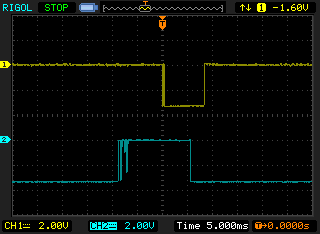
\includegraphics[width=0.5\textwidth]{quadrature_decoder_rigol.png}
\caption{Bounces caused by the mechanical switches of the rotary encoder}
\end{figure}
\begin{figure}
\centering
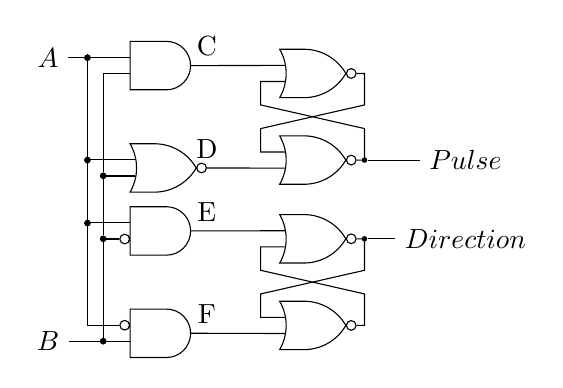
\begin{tikzpicture}[circuit logic US]
\node (A) at (0,1.8) {$A$};
\node (B) at (0,-1.8) {$B$};
\node[branch, draw] at ($(A)+(0.5,0)$) (A1) {};
\node[branch, draw] at ($(A1)+(0,-1.3)$) (A2) {};
\node[branch, draw] at ($(A2)+(0,-0.8)$) (A3) {};
\node[branch, draw] at ($(B)+(0.7,0)$) (B1) {};
\node[branch, draw] at ($(B1)+(0,+1.3)$) (B2) {};
\node[branch, draw] at ($(B2)+(0,+0.8)$) (B3) {};
\node[and gate, draw, inputs=ni] at ($(B2) +(0.7,+0.1)$) (And1) {};
\node[and gate, draw, inputs=in] at ($(B1) +(0.7,+0.1)$) (And2) {};
\node[and gate, draw, inputs=nn] at ($(A1) +(0.9,-0.1)$) (And3) {};
\node[nor gate, draw, inputs=nn] at ($(A2) +(0.9,-0.1)$) (Nor1) {};
\node[nor gate, draw, inputs=nn] at ($(And1) +(1.9,-0.1)$) (Nor2) {};
\node[nor gate, draw, inputs=nn] at ($(And2) +(1.9,+0.1)$) (Nor3) {};
\node[nor gate, draw, inputs=nn] at ($(Nor1) +(1.9,+0.1)$) (Nor4) {};
\node[nor gate, draw, inputs=nn] at ($(And3) +(1.9,-0.1)$) (Nor5) {};
\node (P) at ($(Nor4)+(2,0)$) {$Pulse$};
\node (D) at ($(Nor2)+(2,0)$) {$Direction$};
\draw (A) -- (A1);
\draw (B) -- (B1);
\draw (A1) -- (A2);
\draw (A2) -- (A3);
\draw (B1) -- (B2);
\draw (B2) -- (B3);
\draw (A3) |- (And1.input 1);
\draw (B2) |- (And1.input 2);
\draw (A3) |- (And2.input 1);
\draw (B1) |- (And2.input 2);
\draw (A1) |- (And3.input 1);
\draw (B3) |- (And3.input 2);
\draw (A2) |- (Nor1.input 1);
\draw (B3) |- (Nor1.input 2);
\draw (And1.output) -- +(0.2,0) node[above]{E} -- (Nor2.input 1);
\draw (And2.output) -- +(0.2,0) node[above]{F} -- (Nor3.input 2);
\draw (Nor2.output) -| node[branch] (D1) {} +(0.1,-0.4) -- ($(Nor3) +(-0.6,+0.4)$) |- (Nor3.input 1);
\draw (Nor3.output) -| +(0.1,0.4) -- ($(Nor2) +(-0.6,-0.4)$) |- (Nor2.input 2);
\draw (D1) -- (D);
\draw (And3.output) -- +(0.2,0) node[above]{C} -- (Nor5.input 1);
\draw (Nor1.output) -- +(0,0) node[above]{D} -- (Nor4.input 2);
\draw (Nor5.output) -| +(0.1,-0.4) -- ($(Nor4) +(-0.6,+0.4)$) |- (Nor4.input 1);
\draw (Nor4.output) -| node[branch] (P1) {} +(0.1,0.4) -- ($(Nor5) +(-0.6,-0.4)$) |- (Nor5.input 2);
\draw (P1) -- (P);
\end{tikzpicture}
\caption{Logic gate circuit}
\end{figure}
\begin{figure}
\centering
\begin{tikztimingtable}
A         & LLL N(A1)HHN(A2)L LLL LN(A3)HHN(A4) LLL \\
B         & LLL LN(B1)HHN(B2) LLL N(B3)HHN(B4)L LLL \\
C         & LLL LN(C1)HN(C2)L LLL LN(C3)HN(C4)L LLL \\
D         & HHH N(D1)LLLN(D2) HHH N(D3)LLLN(D4) HHH \\
E         & LLL N(E1)HN(E2)LL LLL LLN(E3)HN(E4) LLL \\
F         & LLL LLN(F1)HN(F2) LLL N(F3)HN(F4)LL LLL \\
Pulse     & LLL LN(P1)HHN(P2) LLL LN(P3)HHN(P4) LLL \\
Direction & LLL LLN(D1)H HHH HHN(D2)L LLL \\
\extracode
\begin{pgfonlayer}{background}
\draw[help lines] (A1) -- (E1);
\draw[help lines] (A2) -- (D1);
\draw[help lines] (A3) -- (P3);
\draw[help lines] (A4) -- (P4);
\draw[help lines] (B1) -- (P1);
\draw[help lines] (B2) -- (P2);
\draw[help lines] (B3) -- (F3);
\draw[help lines] (B4) -- (D2);
\end{pgfonlayer}
\end{tikztimingtable}
\caption{Clean waveforms}
\end{figure}
\begin{figure}
\centering
\begin{BVerbatim}
c <= a and b;
d <= a nor b;
e <= a and not b;
f <= b and not a;
dir <= dir_n nor e;
dir_n <= dir nor f;
pul <= pul_n nor d;
pul_n <= pul nor c;
pulse <= pul;
direction <= dir;
\end{BVerbatim}
\caption{VHDL code of asynchronous design}
\end{figure}
\begin{figure}
\centering
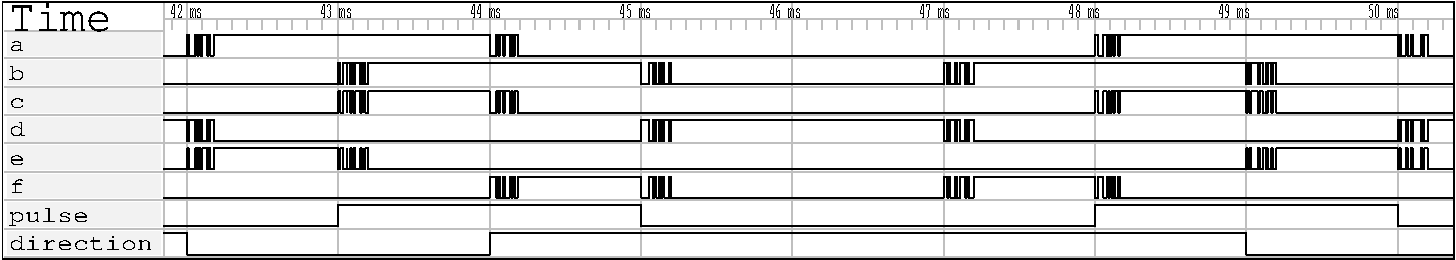
\includegraphics[width=\textwidth]{asynchronous_quadrature_decoder_gtkwave.pdf}
\caption{Waveforms of asynchronous design}
\end{figure}
\begin{figure}
\centering
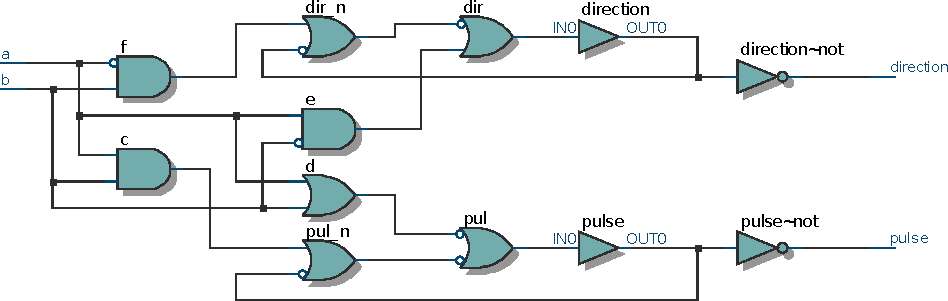
\includegraphics[width=0.5\textwidth]{asynchronous_quadrature_decoder_quartus_rtl.pdf}
\caption{RTL view of asynchronous design}
\end{figure}
\begin{figure}
\centering
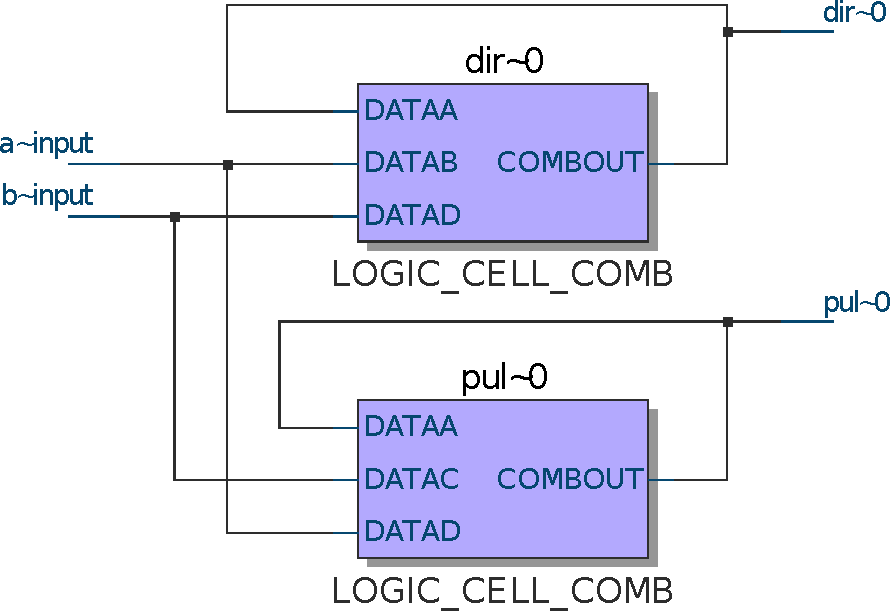
\includegraphics[width=0.5\textwidth]{asynchronous_quadrature_decoder_quartus_map.pdf}
\caption{Reduced to two combinational loops}
\end{figure}
\begin{figure}
\centering
\begin{BVerbatim}
Warning: Found combinational loop of 2 nodes
Warning (332126): Node "decoder_inst|pul~0|dataa"
Warning (332126): Node "decoder_inst|pul~0|combout"
Warning: Found combinational loop of 2 nodes
Warning (332126): Node "decoder_inst|dir~0|dataa"
Warning (332126): Node "decoder_inst|dir~0|combout"
\end{BVerbatim}
\caption{Combinational loop warning}
\end{figure}
\begin{figure}
\centering
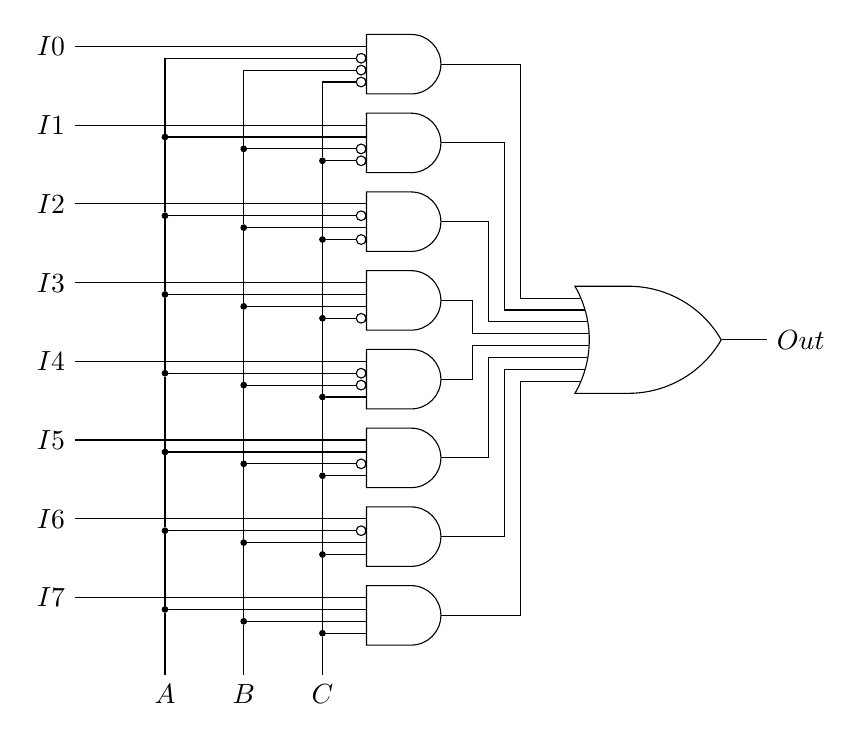
\begin{tikzpicture}[circuit logic US]
\node (A) at (1,0) {$A$};
\node (B) at (2,0) {$B$};
\node (C) at (3,0) {$C$};
\node[and gate, draw, inputs=niii] at (4,8) (And0) {};
\node[and gate, draw, inputs=nnii] at (4,7) (And1) {};
\node[and gate, draw, inputs=nini] at (4,6) (And2) {};
\node[and gate, draw, inputs=nnni] at (4,5) (And3) {};
\node[and gate, draw, inputs=niin] at (4,4) (And4) {};
\node[and gate, draw, inputs=nnin] at (4,3) (And5) {};
\node[and gate, draw, inputs=ninn] at (4,2) (And6) {};
\node[and gate, draw, inputs=nnnn] at (4,1) (And7) {};
\node[or gate, draw, inputs=nnnnnnnn] at (7,4.5) (Or0) {};
\node (O) at ($(Or0.output)+(1,0)$) {$Out$};
\node (I0) at ($(And0.input 1)+(-4,0)$) {$I0$};
\node (I1) at ($(And1.input 1)+(-4,0)$) {$I1$};
\node (I2) at ($(And2.input 1)+(-4,0)$) {$I2$};
\node (I3) at ($(And3.input 1)+(-4,0)$) {$I3$};
\node (I4) at ($(And4.input 1)+(-4,0)$) {$I4$};
\node (I5) at ($(And5.input 1)+(-4,0)$) {$I5$};
\node (I6) at ($(And6.input 1)+(-4,0)$) {$I6$};
\node (I7) at ($(And7.input 1)+(-4,0)$) {$I7$};
\node[branch, draw] at ($(And1.input 2 -| A)$) (A1) {};
\node[branch, draw] at ($(And1.input 3 -| B)$) (B1) {};
\node[branch, draw] at ($(And1.input 4 -| C)$) (C1) {};
\node[branch, draw] at ($(And2.input 2 -| A)$) (A2) {};
\node[branch, draw] at ($(And2.input 3 -| B)$) (B2) {};
\node[branch, draw] at ($(And2.input 4 -| C)$) (C2) {};
\node[branch, draw] at ($(And3.input 2 -| A)$) (A3) {};
\node[branch, draw] at ($(And3.input 3 -| B)$) (B3) {};
\node[branch, draw] at ($(And3.input 4 -| C)$) (C3) {};
\node[branch, draw] at ($(And4.input 2 -| A)$) (A4) {};
\node[branch, draw] at ($(And4.input 3 -| B)$) (B4) {};
\node[branch, draw] at ($(And4.input 4 -| C)$) (C4) {};
\node[branch, draw] at ($(And5.input 2 -| A)$) (A5) {};
\node[branch, draw] at ($(And5.input 3 -| B)$) (B5) {};
\node[branch, draw] at ($(And5.input 4 -| C)$) (C5) {};
\node[branch, draw] at ($(And6.input 2 -| A)$) (A6) {};
\node[branch, draw] at ($(And6.input 3 -| B)$) (B6) {};
\node[branch, draw] at ($(And6.input 4 -| C)$) (C6) {};
\node[branch, draw] at ($(And7.input 2 -| A)$) (A7) {};
\node[branch, draw] at ($(And7.input 3 -| B)$) (B7) {};
\node[branch, draw] at ($(And7.input 4 -| C)$) (C7) {};
\draw (I0) -- (And0.input 1);
\draw (I1) -- (And1.input 1);
\draw (I2) -- (And2.input 1);
\draw (I3) -- (And3.input 1);
\draw (I4) -- (And4.input 1);
\draw (I5) -- (And5.input 1);
\draw (I6) -- (And6.input 1);
\draw (I7) -- (And7.input 1);
\draw (A1) |- (And0.input 2);
\draw (B1) |- (And0.input 3);
\draw (C1) |- (And0.input 4);
\draw (A1) -- (And1.input 2);
\draw (B1) -- (And1.input 3);
\draw (C1) -- (And1.input 4);
\draw (A2) -- (And2.input 2);
\draw (B2) -- (And2.input 3);
\draw (C2) -- (And2.input 4);
\draw (A3) -- (And3.input 2);
\draw (B3) -- (And3.input 3);
\draw (C3) -- (And3.input 4);
\draw (A4) -- (And4.input 2);
\draw (B4) -- (And4.input 3);
\draw (C4) -- (And4.input 4);
\draw (A5) -- (And5.input 2);
\draw (B5) -- (And5.input 3);
\draw (C5) -- (And5.input 4);
\draw (A6) -- (And6.input 2);
\draw (B6) -- (And6.input 3);
\draw (C6) -- (And6.input 4);
\draw (A7) -- (And7.input 2);
\draw (B7) -- (And7.input 3);
\draw (C7) -- (And7.input 4);
\draw (A) -- (A7);
\draw (B) -- (B7);
\draw (C) -- (C7);
\draw (A1) -- (A2);
\draw (B1) -- (B2);
\draw (C1) -- (C2);
\draw (A2) -- (A3);
\draw (B2) -- (B3);
\draw (C2) -- (C3);
\draw (A3) -- (A4);
\draw (B3) -- (B4);
\draw (C2) -- (C4);
\draw (A4) -- (A5);
\draw (B4) -- (B5);
\draw (C4) -- (C5);
\draw (A5) -- (A6);
\draw (B5) -- (B6);
\draw (C5) -- (C6);
\draw (A6) -- (A7);
\draw (B6) -- (B7);
\draw (C6) -- (C7);
\draw (And0.output) -- +(1,0) |- (Or0.input 1);
\draw (And1.output) -- +(0.8,0) |- (Or0.input 2);
\draw (And2.output) -- +(0.6,0) |- (Or0.input 3);
\draw (And3.output) -- +(0.4,0) |- (Or0.input 4);
\draw (And4.output) -- +(0.4,0) |- (Or0.input 5);
\draw (And5.output) -- +(0.6,0) |- (Or0.input 6);
\draw (And6.output) -- +(0.8,0) |- (Or0.input 7);
\draw (And7.output) -- +(1,0) |- (Or0.input 8);
\draw (Or0.output) -- (O);
\end{tikzpicture}
\caption{Lookup table logic circuit}
\end{figure}
\begin{figure}
\centering
\begin{tikztimingtable}[xscale=0.25]
I0  & 200H \\
I1  & 200L \\
I2  & 200H \\
I3  & 200L \\
I4  & 200L \\
I5  & 200L \\
I6  & 200L \\
I7  & 200L \\
A   & 25L 25H N(A1) 25L 25H N(A2) 25L 25H 25L 25H \\
B   & 51L 50H N(B1) 50L 49H \\
C   & 102L 98H \\
Out & 25H 25L N(O1)25H 25L N(O2)HN(O3) 24L 25L 25L 25L \\
\extracode
\begin{pgfonlayer}{background}
\draw[help lines] (A1) -- (O1);
\draw[help lines] (A2) -- (O2);
\draw[help lines] (B1) -- (O3);
\end{pgfonlayer}
\end{tikztimingtable}
\caption{Glitch on output when multiple inputs change at almost the same time}
\end{figure}
\begin{figure}
\centering
\begin{BVerbatim}
c <= a xor b;
dir <= b when rising_edge(clock) and c = '1' else dir;
pul <= a when rising_edge(clock) and c = '0' else pul;
pulse <= pul;
direction <= dir;
\end{BVerbatim}
\caption{VHDL code of synchronous design}
\end{figure}
\begin{figure}
\centering
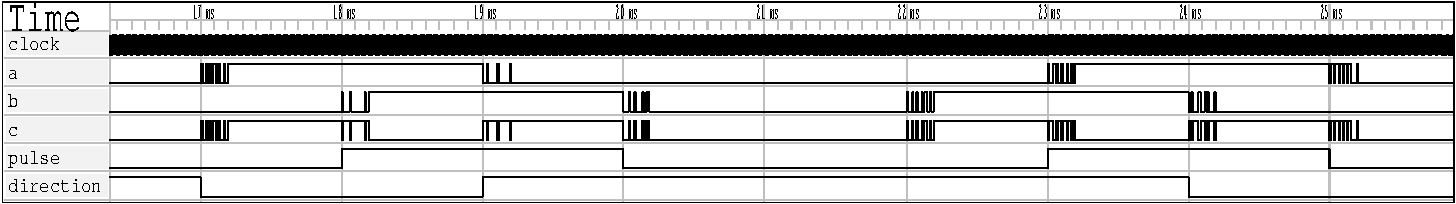
\includegraphics[width=\textwidth]{quadrature_decoder_gtkwave.pdf}
\caption{Waveforms of synchronous design}
\end{figure}
\begin{figure}
\centering
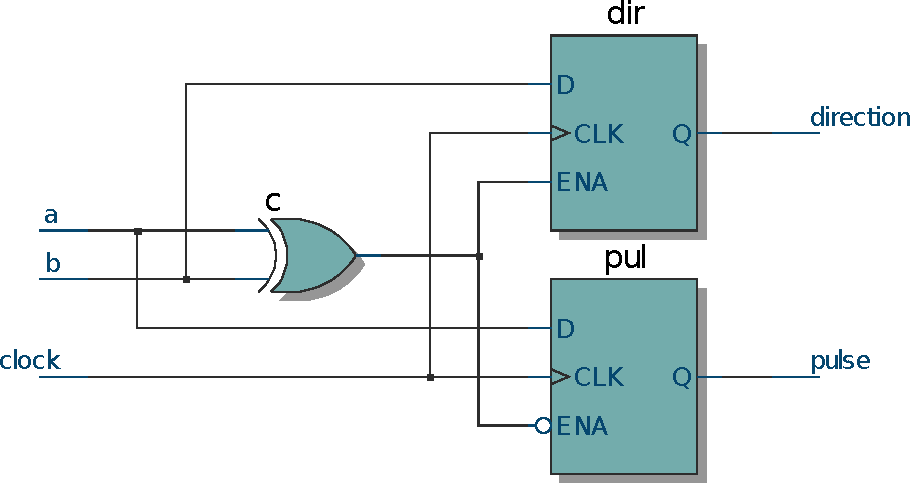
\includegraphics[width=0.5\textwidth]{quadrature_decoder_quartus_rtl.pdf}
\caption{RTL view of synchronous design}
\end{figure}
\begin{figure}
\centering
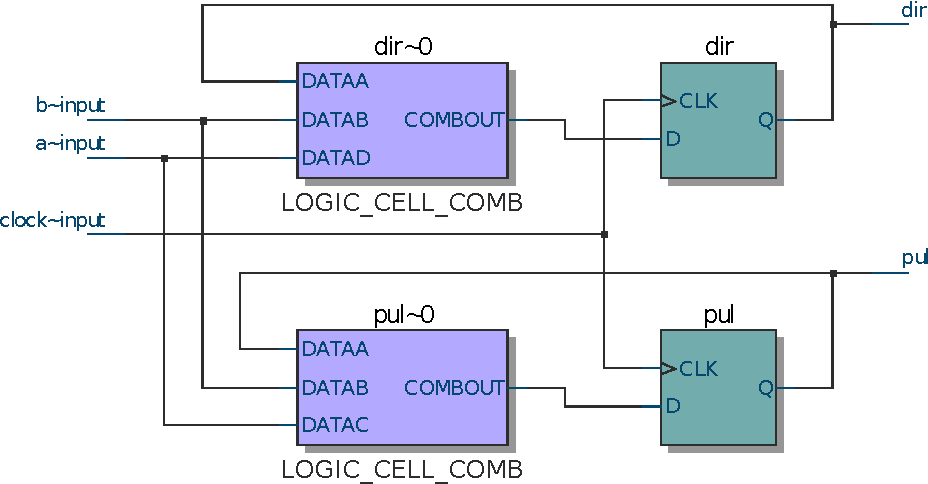
\includegraphics[width=0.5\textwidth]{quadrature_decoder_quartus_map.pdf}
\caption{Technology map view of synchronous design}
\end{figure}
\end{document}
